\documentclass[a4paper,12pt]{article}
\usepackage{amsmath,amsfonts,amsthm,amscd,amssymb,latexsym}%,eufrak}
%%%%%%%%%%%%%
\usepackage{caption}
\usepackage{subcaption}
\usepackage{enumerate,graphicx,psfrag}%,subfigure}%,jchangebar,oldgerm}
\usepackage[mathscr]{eucal}
\usepackage[usenames]{color}
\usepackage{url}
\usepackage[shortlabels]{enumitem}
\usepackage{comment}
%\usepackage[utf8]{inputenc}
\usepackage[T1]{fontenc}
%\usepackage{showkeys}
\usepackage{wrapfig}
\usepackage{lscape}
\usepackage{rotating}
%%%%%%%%%
\sloppy
%%%%%%%%%%%%%%%%%%%%%%%
\title{The subgroup membership problem in amalgamated products of 
finitely generated free groups
}
\author{Andrew J. Duncan, Elizaveta Frenkel}

\renewcommand{\a}{\alpha }
\renewcommand{\b}{\beta }
\newcommand{\G}{\Gamma }
\newcommand{\g}{\gamma }
\newcommand{\D}{\Delta }
\renewcommand{\d}{\delta }
%\def\vd{\vardelta}
\newcommand{\ep}{\epsilon }
\newcommand{\e}{\varepsilon }
\newcommand{\z}{\zeta }
%\eta
\renewcommand{\th}{\theta }
\newcommand{\T}{\Theta }
\renewcommand{\i}{\iota }
\renewcommand{\k}{\kappa }
\renewcommand{\l}{\lambda }
\renewcommand{\L}{\Lambda }
%\mu
%\nu
%\xi
%omicron
%\pi
\renewcommand{\r}{\rho }
\newcommand{\s}{\sigma }
\renewcommand{\S}{\Sigma }
\renewcommand{\t}{\tau }
\newcommand{\up}{\upsilon }
\newcommand{\U}{\Upsilon }
%\phi
\newcommand{\x}{\chi }
%\psi
\newcommand{\W}{\Omega }
\newcommand{\w}{\omega }
%%%%%%%%%%%%%%%%%%%%%%%%%%%%%%%
%%%%%%%%%%%%%%%%%%%%%%%%%%%%%
\newcommand{\pd}{\partial}
\newcommand{\wht}{\widehat}
%\newcommand{\cC}{{\mathcal C}}
%\newcommand{\cdim}{\texttt{cdim}}
\newcommand{\fC}{{\textswab C}}
\newenvironment{ef}{\noindent\color{blue} \bf EF: }{}
%
\newcommand{\cA}{{\cal{A}}}
\newcommand{\cD}{{\cal{D}}}
\newcommand{\cF}{{\cal{F}}}
\newcommand{\cH}{{\cal{H}}}
\newcommand{\cJ}{{\cal{J}}}
\newcommand{\cK}{{\cal{K}}}
\newcommand{\cP}{{\cal{P}}}
\newcommand{\cQ}{{\cal{Q}}}
\newcommand{\cR}{{\cal{R}}}
\newcommand{\cS}{{\cal{S}}}
\newcommand{\cV}{{\cal{V}}}
\newcommand{\cW}{{\cal{W}}}
%\newcommand{\GG}{\ensuremath{\mathbb{G}}}
\newcommand{\pp}{\mathbf{p}}
%%%%%%%%%%%%%%%%%%%%%%%%%%%%%%
\newcommand{\nul}{\emptyset }
\newcommand{\vim}{\nu\textrm{-im}}
%%%%%%%%%%%%%%%%%%%%%%%%%%%%%%
\newtheorem{theorem}{Theorem}[section]
\newtheorem{lemma}[theorem]{Lemma}
\newtheorem{corollary}[theorem]{Corollary}
\newtheorem{proposition}[theorem]{Proposition}
\newtheorem{axiom}[theorem]{Axiom}
\newtheorem{definition}[theorem]{Definition}
\newtheorem*{defn*}{Definition}
\newtheorem{conjecture}[theorem]{Conjecture}
%cvs -d :pserver:najd2@cvs.mas.ncl.ac.uk:/CVS/najd2
\newtheorem{exam}[theorem]{Example}
%\newtheorem{comment}[theorem]{Comment}
%
%
\newenvironment{example}{\begin{exam} \rm}{\end{exam}}
%
%
%
\newtheorem{remk}[theorem]{Remark}
\newenvironment{remark}{\begin{remk} \rm}{\end{remk}}
%
%%%%%%%%%%%%
\numberwithin{equation}{section}
\numberwithin{figure}{section}
%%%%%%%%%%%%%%%%%%%%
\newcommand{\Loop}{\operatorname{Loop}}
\newcommand{\Iso}{\operatorname{Isom}}
\newcommand{\Aut}{\operatorname{Aut}}
%%%%%%%%%%%%%%%%%%%
\renewcommand{\AA}{\ensuremath{\mathbb{A}}}
\newcommand{\ZZ}{\ensuremath{\mathbb{Z}}}
\newcommand{\QQ}{\ensuremath{\mathbb{Q}}}
\newcommand{\RR}{\ensuremath{\mathbb{R}}}
\newcommand{\NN}{\ensuremath{\mathbb{N}}}
\newcommand{\CC}{\ensuremath{\mathbb{C}}}
\newcommand{\FF}{\ensuremath{\mathbb{F}}}
%\renewcommand{\ker}{\verb"Ker"}
\newcommand{\cC}{\mathcal{C}}
\renewcommand{\cF}{\mathcal{F}}
\newcommand{\cO}{\mathcal{O}}
\renewcommand{\cS}{\mathcal{S}}
\newcommand{\la}{\langle}
\newcommand{\ra}{\rangle}
%\newcommand{\BA}{\ensuremath{\mathbb{A}}}
%%%%%%%%%%%%%%%%%%%%%%%%%%%%%%%%%%%%%%
\newcommand{\maps}{\rightarrow}
\newcommand{\ov}[1]{\overline{#1}}
\newcommand{\bs}{\backslash}
%%%%%%%%%%%%%%%%%%%%%%%%%%%%%%%
\newcommand{\be}{\begin{enumerate}}
\newcommand{\ee}{\end{enumerate}}
\newcommand{\bd}{\begin{description}}
\newcommand{\ed}{\end{description}}
\newcommand{\biz}{\begin{itemize}}
\newcommand{\eiz}{\end{itemize}}
%%%%%%%%%%%%%%%%%%%%%%%%%%%%%%%%%%%
%
\newenvironment{ajd1}{\noindent\color{red} AJD }{}
\newcommand{\ajd}[1]{\begin{ajd1} #1 \end{ajd1}}
%
%\includecomment{comp}% to see environment comp
\excludecomment{comp}% to hide environment comp
%
\begin{document}
$F_1=F( x_1,x_2)$, $F_2=F(y_1, y_2)$, $H_1=\la x_2x_1^{-1}, x_2^3, x_2x_1x_2,
x_1^{-1}x_2\ra$, $H_2$ is the same with $y_1$ instead of $x_1$ and $y_2$ instead
of $x_2$. $\phi_1$ maps $z_1$ to $  x_2x_1^{-1}$, $z_2$ to $x_2^3$, $z_3$ to 
 $x_2x_1x_2$ and $z_4$ to $x_1^{-1}x_2$. $\phi_2$ does the same but 
with $y_i$ in place of $x_i$. $H_k$ is normal in $F_k$.
The Stallings folding for $H_1$ is shown in figure \ref{fig:fold}.
\begin{figure}
\begin{center}
\psfrag{a1}{$x_1|z_1^{-1}$}
\psfrag{a2}{$x_1|z_3$}
\psfrag{a3}{$x_1|z_4^{-1}$}
\psfrag{b1}{$x_2|1$}
\psfrag{b2}{$x_2|z_2$}
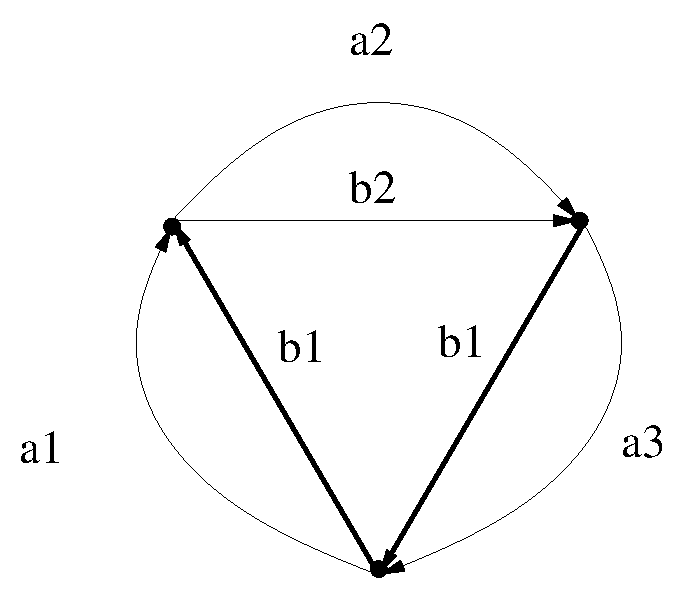
\includegraphics[scale=0.6]{ce.eps}
\caption{}\label{fig:fold}
\end{center}
\end{figure}
\\[1em]

\par\noindent $K=\la y_1x_1,x_1^{-1}x_2\ra$. \\[1em]
$K\cap H_1$ contains $y_1x_1$ and, for all $n>0$, $K$ contains
\[(y_1x_1)^{-n}(x_1^{-1}x_2)(y_1x_1)^{n}=x_1^{-2n}(x_1^{-1}x_2) x_1^{2n},\]
and 
\[(y_1x_1)^{n}(x_1^{-1}x_2)(y_1x_1)^{-n}=x_1^{2n-1}(x_2x_1^{-1}) x_1^{-(2n-1)},\]
both of which follow by induction on $n$, using the fact that $H_i$ is normal. 
As $H_1$ is normal both of these are in fact in $K\cap H_1$. \\[1em]
Therefore, for all $n\in \ZZ$, $K\cap H_1$ contains $x_1^{-2n}(x_1^{-1}x_2) x_1^{2n}$. \\[1em]
Let $L=\la x_1^{-2n}(x_1^{-1}x_2) x_1^{2n}|n\in \ZZ\ra$. Then, again by induction, 
\[L=\{x_1^{2n_1}(x_1^{-1}x_2)^{r_1}\cdots (x_1^{-1}x_2)^{r_k}x_1^{2n_{k+1}}\,|\,n_i,r_i\in\ZZ, \sum n_i=0\}\]
and also $L$ is normal in $K$, as $(y_1x_1)^{-1}(x_1^{-2n}(x_1^{-1}x_2) x_1^{2n})(y_1x_1)^{-1}\in L$.  
The subgroup $\la y_1x_1\ra$ has elements with reduced (amalgam) form $(y_1x_1)^n$ and none 
of these belong to a factor, except when $n=0$, so $L\cap \la y_1x_1\ra=\{1\}$. Therefore
$K=L\rtimes \la y_1x_1\ra$, the internal semi-direct product of $L$ and $\la y_1x_1\ra$.
The intersection of $K$ and $H_1$ can be seen to be $L$ and  representatives for all 
elements of $L$ are required. 
Figure \ref{fig:Kfold_inf}, which shows an folded automaton for $K$. If $y_1$ is deleted from
this then a  Stallings folding for the subgroup $L$ of $F_1$ is left, so $L$ has infinite
rank in $F_1$. This means infinitely many representatives for elements of $L$ will 
be needed. 
\begin{figure}
\begin{center}
\psfrag{x1}{$x_1$}
\psfrag{x2}{$x_2$}
\psfrag{y1}{$y_1$}
\psfrag{1}{$1$}
\includegraphics[scale=0.4]{Kfold_inf.eps}
\caption{}\label{fig:Kfold_inf}
\end{center}
\end{figure}
%\bibliographystyle{plain}
%\bibliography{membership}
\end{document}